\section{Prototype - System for Data Collection}
\label{sec:wireframes}

  This section will provide a proposed system for data collection. First we will look at a framework for evaluating the usability of the system for data collection in Section~\ref{sec:usability}. The design choices and the wireframes for the system are described and illustrated in Section~\ref{sec:designChoices}.

  \subsection{Usability} \label{sec:usability}

  When creating a system it is important to evaluate its usability. This section will provide a framework to include when designing the a prototype for data collection. The prototype is further the described and illustrated in the next section.

  Usability is defined as ``the extent to which a product can be used by specified users to achieve specified goals with effectiveness, efficiency and satisfaction in a specified context of use'' \cite{ISO9241}. Figure~\ref{fig:usability} is showing how we are going to measure the usability of the prototype created for data collection.

  The first level contains the usability measures effectiveness, efficiency, and satisfaction. The first usability measure, {\it efficiency}, is defined as ``resources expended in relation to the accuracy and completeness with which users achieve goals'' and is measured at the usability metric time on task. The second usability measure, {\it effectiveness}, is defined as ``the accuracy and completeness with which users achieve specified goals'' and is measured by the usability metrics number of errors and completion rate. The last usability measure, {\it satisfaction}, is defined as ``freedom from discomfort and positive attitudes towards the use of the product. '' and is measured by the usability metric of subjective satisfaction.

  \begin{figure}[H]
    \centering
    \includegraphics[scale=0.25]{pics/usability.png}
    \caption[ISO9241 - Usability]{ISO9241 - Usability \cite{ISO9241}}
    \label{fig:usability}
  \end{figure}

  The prototype that is being evaluated is a prototype for data collection, e.g., the system. A user is defined as ``the persons who interact with the product'' and is the respondents that answer the survey through the system. The goal of the system is to collect patterns and information about the users. The task that the respondents needs to perform is to provide their answers to the questions asked in the questionnaire (Section~\ref{sec:questions}). The product, for which usability is to be evaluated, is the prototype for the software being implemented on mobile devices.  

  \subsection{Design choices} \label{sec:designChoices}
    
  This section will be a proposal for how we can build a system for data collection. The system is a prototype of the questionnaire, and will be created as a web application that will be easy to distribute over the Internet. This is only a proposal for a system, and the final system will be implemented next semester. During this project, I have spent much time designing the look and feel of the system, as well as the structure and flow. The final system will only be running on a smartphone.

  When designing a system for a mobile device, there is many usability requirements that must be considered (Figure~\ref{fig:usability}). {\it First}, the system must be efficient to use. When interacting with a small screen, I need to consider how the respondent can complete the questionnaire as fast as possible. The number of questions is quite high, therefore, we need to establish a flow that supports the user to complete the questionnaire quickly. It is not desired to get in a situation where many of the respondents quit before finishing the questionnaire because it takes too long time. {\it Second}, the system need to be effective in terms of the respondent's completion rate, avoiding too many errors. When considering the effectiveness of the systems, the system needs to support the respondents to be able to complete the questionnaire. {\it Third}, when using the system, the respondents need to get a positive attitude towards using the system. This usability requirement is often used to design systems that people want to use. For this system, it may not be a system that people find fun to use, but maybe I am able to design it in a way that people find it interesting. It should also be considered that the respondents feel confident while using the system. The system are collecting patterns created by the respondent, making the system be considered as trustworthy in order to reach a subjective satisfaction from the respondents.

  When designing the system, the first issue was to design the response alternatives and how the respondents efficiently select their answer. For illustrating the answers, I picked out icons that I believe have a universal semantic meaning. By universal semantic meaning, I am talking about icons that people of different ages and different nationalities are familiar with. To illustrate one example, I used an image of a girl and a boy that is usually used on for example toilets (Figure~\ref{fig:boygirl}). When the user is asked for their gender, the two images are visualized as the possible alternatives instead of using text. Using too much text can take too much time to interpret, as well as it might keep the respondent attention throughout the whole questionnaire by using visual alternatives. I also believe that using universal icons support respondents that are not fluent in English to be able to answer the questionnaire.

  \begin{figure}[H]
    \centering
    \subfigure[Male]{
      \includegraphics[scale=0.5]{pics/male3.png}
    }
    \subfigure[Female]{
      \includegraphics[scale=0.5]{pics/female3.png}
    }
    \caption{Icons used for illustrate the gender alternatives}
    \label{fig:boygirl}
  \end{figure}

  Since this system only is supposed to be answered by a mobile device, the only input is coming from the touch screen. When the alternatives for each question are illustrated with icons, it is very easy for the respondents to select their answers by clicking on the icon. This helps the users to choose their answers quickly. Other aspects are the error rate and completion rate when looking at the usability measure effectiveness. The icons are easy to interact with from a touch screen. Other alternatives for the respondents to select their answer could be a list of textual alternatives. Such icons are called radio buttons and are often small. This can cause a situation where a person selects an answer that was not intended. I believe that using big icons can reduce the error rate, as well as raise the completion rate. This might also increase the subjective satisfaction because it may avoid an annoying situation where it takes too long time to interpret the alternatives, as well as avoid misplaced answers.

  When answering a questionnaire it is important to indicate the progress, e.g. how far the respondent is from completion. This will support the satisfaction of the user. The progress can be illustrated with a progress bar or percentage/number of completed answers. If there is no indication of the progress, there is not added any ``award'' for answering each question. When the respondents can see the progress for each completed answer, they may feel that they were getting an award and therefore feeling satisfied.

  The flow and structure are also an important aspect of usability. As stated, the respondents should be able to complete the questionnaire as fast as possible. When designing the wireframes for the prototype, it is hard to use flow elements that often is used on mobile devices. Such elements are animation and automatic progress. I have chosen to use arrows to support the flow and progress in the prototype because other features is hard to illustrate on paper. The flow is, therefore, added to further discussion in Chapter~\ref{chap:FutureWork}.

  The next section will include the wireframes for the prototype. Figure~\ref{fig:navigation} is four of the icons used in the wireframes for the navigation and progress. Figure~\ref{fig:left} and Figure~\ref{fig:right} is the navigation elements used for progressing trough the system. Figure~\ref{fig:help} is an icon used if the respondent does not understand the question, and will provide extended information. Figure~\ref{fig:progress} is the progress bar indicating the progress in the questionnaire. 

  \begin{figure}[H]
    \centering
    \subfigure[Navigate left]{
      \includegraphics[scale=1]{pics/leftarrow5.png}
      \label{fig:left}
    }
    \subfigure[Help]{
      \includegraphics[scale=0.16]{pics/question48.png}
      \label{fig:help}
    }
    \subfigure[Navigate right]{
      \includegraphics[scale=1]{pics/rightarrow6.png}
      \label{fig:right}
    }
    \subfigure[Progress]{
      \includegraphics[scale=1.15]{pics/progress.png}
      \label{fig:progress}
    }
    \caption{Navigation elements}
    \label{fig:navigation}
  \end{figure}

  \subsection{Wireframing - Designing the prototype}

    The prototype is created with a method called wireframing. A wireframe is low-fidelity prototype design that is sketchy and incomplete. Wireframes are easily constructed at a low cost and is made to avoid design issues when implementing the final system. The wireframes are the first proposal for the data collection system and will be used to test broad concepts of the prototype before the implementation.

  The wireframes in the next section are at version 3 and have been through several reviews. First, I contacted created the first version by mocking up a design. {\it Second}, I contacted an assistant professor, Ole Andreas Alsos, from Department of Computer and Information Science at my university. He also teaching in a course named ``Prototyping Interactive Media'' (TDT4262). I scheduled a meeting with Ole Andreas to get feedback on the first version of the prototype. After the meeting I got much feedback on how to ask questions, as well as feedback on the overall design. This led to the version 2 of the prototype.

  In December 8-10, my co-supervisor, Per Thorsheim, arranged a conference called ``PasswordsCon'' \cite{conference} at my university. At the conference, there were participants from all over the world; all with the same interest in passwords. For me, this was an excellent opportunity for me to talk to researchers and other people with an interest in passwords. Here I met one of the researchers that published the first large-scale user study on the Android Unlock Patten, Markus Dürmuth \cite{Uellenbeck}. I also met a researcher from Cambridge University, Jeunese Payne, that interested in passwords and psychology. Her main field of study is psychology, but she recently works on a project called ``Pico'' at Cambridge University that investigate a new authentication scheme. I sat down with both Markus and Jeunese, and explained my research and the selected research design that is described in this chapter. They both provided feedback on the wireframes and the overall research. At the same conference, I also presented this project thesis \cite{presentation}. The conference was an important event for this research as I got many responses from researchers that were interested in the work I am doing in my master thesis. I got much motivation, as well as retrieved a bigger network of password interested people from all over the world. This will be an important network to have when I am going to collect the data in the next semester.

  At the end of the conference, I gathered the feedback that resulted in version 3 of the wireframes. The final version is described in detail in the next section.

  \subsection{Wireframes} \label{sec:thewireframes}

  This section includes a description of the prototype for data collection illustrated in wireframes.   

    \begin{wrapfigure}{l}{0.35\textwidth}
      \centering
      \vspace{-5pt}
      \includegraphics[scale=0.40]{screens/v3/mobile/mobile1-1.png}
      \caption{Introduction screen}
      \label{fig:wireframe1}
    \end{wrapfigure}

  Figure~\ref{fig:wireframe1} is the first screen that the respondents meet when they access the questionnaire. This includes a description of the research, information about the questionnaire, and privacy concerns for the respondent. This is the first part that the respondents meet, so it is important that the defendant feel confident. The contact information provides a creditability to the questionnaire, so the respondents can feel save that information is handled correctly accordingly to the information that is given. It also allows the respondents to ask questions if they have any questions or want to Google the researcher responsible for questionnaire. A questionnaire asking for personal information might seem scary for some respondents, it is then comforting to be able to see who this person is.

  When the respondents are decided to participate, they press start and is transferred to the screen in Figure~\ref{fig:wireframe2}. This screen is providing information about the Android Unlock Patten, so they can know how to type the pattern. If the respondents have not tried the unlock pattern before, they will get the choice to try the scheme before entering their pattern. For experienced users, they can skip the training for saving time. Figure~\ref{fig:wireframe3} shows the training mode. The registered patterns are collected to be able to compare the pattern in the training mode, as well as the selected patterns. Figure~\ref{fig:wireframe4} is the start screen for the pattern creation. The respondents are asked to make three patterns, one for a shopping account, one pattern for their smartphone, and one pattern for their banking account.

    \begin{figure}[H]
      \subfigure[Introduction to Android Lock Pattern]{
        \includegraphics[scale=0.48]{screens/v3/plain/plain1-2.png}
        \label{fig:wireframe2}
      }
      \subfigure[Training mode]{ 
        \includegraphics[scale=0.48]{screens/v3/plain/plain1-3.png}
        \label{fig:wireframe3}
      }
      \subfigure[Introduction to pattern creation]{
        \includegraphics[scale=0.48]{screens/v3/plain/plain1-4.png}
        \label{fig:wireframe4}
      }
    \end{figure}

  The pattern creation is showed in Figure~\ref{fig:wireframe5}, Figure~\ref{fig:wireframe6}, and Figure~\ref{fig:wireframe7}. For different users, the order of the different pattern will occur in a different order using the Latin Square method that was described in Section~\ref{sec:layout}.

    \begin{figure}[H]
      \subfigure[Creation of pattern 1]{
        \includegraphics[scale=0.48]{screens/v3/plain/plain1-5.png}
        \label{fig:wireframe5}
      }
      \subfigure[Creation of pattern 2]{
        \includegraphics[scale=0.48]{screens/v3/plain/plain1-6.png}
        \label{fig:wireframe6}
      }
      \subfigure[Creation of pattern 3]{
        \includegraphics[scale=0.48]{screens/v3/plain/plain1-7.png}
        \label{fig:wireframe7}
      }
    \end{figure}

  The first part have focused on the pattern creation because it is the most crucial information needed. After the pattern creation, the questionnaire will now ask the respondents about demographic, experience and use of lock screens and some information about the device used to answer the questionnaire. All of these questions is found in Table~\ref{tab:questions}, and most of the human properties is found in the analysis of human properties in Section~\ref{sec:datarequirements}.

  Figure~\ref{fig:wireframe8} is asking about the respondent's hand size. The answers from this question will be subjective, but there is not any other way this can be asked. Asking people to measure the actual size would be preferable but would require too much time for the respondents. They also might not have any instruments available to measure their precise length. Figure~\ref{fig:wireframe9} is asking the respondents about their screen size. This will also be subjective. In order to be able to get the correct size, there will be used JavaScript to detect the actual size of the screen in (illustrated in Listing~\ref{list:screen}). Why add a question that is possible to detect automatically? It is not desired to collect data that is not explicitly asked.

  \medskip
  \begin{lstlisting}[caption=Detecting screen size in JavaScript, label=list:screen]
    var height = window.screen.availHeight;
    var width = window.screen.availWidth;
  \end{lstlisting}

  In Figure~\ref{fig:wireframe10} it is asked for the hand used when the respondent answered the questionnaire. This can be used when predicting the likely initial starting point that was discussed in Section~\ref{sec:datarequirements}

    \begin{figure}[H]
    \ContinuedFloat
      \subfigure[Q1: Hand size]{
        \includegraphics[scale=0.48]{screens/v3/plain/plain2-1.png}
        \label{fig:wireframe8}
      }
      \subfigure[Q2: Screen size]{
        \includegraphics[scale=0.48]{screens/v3/plain/plain2-2.png}
        \label{fig:wireframe9}
      }
      \subfigure[Q3: Handedness]{
        \includegraphics[scale=0.48]{screens/v3/plain/plain2-3.png}
        \label{fig:wireframe10}
      }
    \end{figure}

    When the respondent is using either left- or right-hand, it is crucial to know the finger used (Figure~\ref{fig:wireframe11}). If the respondent is using their thumb, it is likely that they held the smartphone in one hand. If the forefinger is used, it is likely that the respondent used the forefinger. My hypothesis is that this is necessary information to collect because the finger used is deciding which part of the screen they can reach. In the next wireframe the respondent is asked about their reading direction (Figure~\ref{fig:wireframe12}). The most common reading direction in most countries is from left to right. People using Arabic for reading and writing usually have the right-to-left direction. Some countries in Asia (Japan, Korea, China, and Taiwan) is reading and writing from top-to-bottom, left-to-right. 
    The next information is about the user's gender, and is illustrated in Figure~\ref{fig:wireframe13}.

    \begin{figure}[H]
    \ContinuedFloat
      \subfigure[Q4: Finger used in pattern creation]{
        \includegraphics[scale=0.48]{screens/v3/plain/plain2-4.png}
        \label{fig:wireframe11}
      }
      \subfigure[Q5: Reading/Writing orientation]{
        \includegraphics[scale=0.48]{screens/v3/plain/plain2-5.png}
        \label{fig:wireframe12}
      }
      \subfigure[Q6: Gender]{
        \includegraphics[scale=0.48]{screens/v3/plain/plain2-6.png}
        \label{fig:wireframe13}
      }
    \end{figure}

    When collecting demographics, it is important to know the age of the respondents. It is not known if it will give any results that can be shown to be statistically significant, but it is desired to be able to have a diversity in the age of the respondents. There might be some difference in the risk awareness, or the experience with mobile phones. The age is not grouped into different interval because it is hard to predict reasonable age interval of the sample (Figure~\ref{fig:wireframe14}). The nationality is important to have so it is possible to see how the data is represented on the map. When making statistical tests, it is important to be able to reason about its representation worldwide, or if the results only statistical significant for some part of the world. It is desired to collect data from different nationalities. The respondents selects their nationality from a list. The list might be quite long. To make it easier for the respondents to answer it is possible to map their browser language to their nationality and put them on top of the list. Many respondents might use English as their preferred browser language, then it is not very easy to list specific nationalities on the top of the list. The JavaScript code is illustrated in Listing~\ref{list:language} and the wireframe is illustrated in Figure~\ref{fig:wireframe15}. 

    \medskip
    \begin{lstlisting}[caption=Detecting browser language, label=list:language]
      var browser_language;
      if (navigator.userLanguage) // IE
        browser_language = navigator.userLanguage;
      else if (navigator.language) // FF, Chrome, Safari, Opera
        browser_langauge = navigator.language;
    \end{lstlisting}

    The next wireframe there is a question about whether they have used the Android Unlock Pattern or not (Figure~\ref{fig:wireframe16}). This information can be used to compare respondents that have used the scheme before and those who have not. 

    \begin{figure}[H]
      \ContinuedFloat
      \subfigure[Q7: Age]{
        \includegraphics[scale=0.48]{screens/v3/plain/plain2-7.png}
        \label{fig:wireframe14}
      }
      \subfigure[Q8: Nationality]{
        \includegraphics[scale=0.48]{screens/v3/plain/plain2-8.png}
        \label{fig:wireframe15}
      }
      \subfigure[Q9: Android Unlock Pattern experience]{
        \includegraphics[scale=0.48]{screens/v3/plain/plain2-9.png}
        \label{fig:wireframe16}
      }
    \end{figure}

    Figure~\ref{fig:wireframe17} is asking if the respondents use a screen lock, and if they do, they are redirected to Figure~\ref{fig:wireframe18}. If not, they are directly directed to Figure~\ref{wireframe19}. Figure~\ref{fig:wireframe19} is asking about the mobile Operating System (abbreviated OS) on the mobile used for answering the questionnaire. This is a tricky question to ask because there might be many people that don't know what an operating system is. There are different ways to collect the operating system of the mobile used:

      \begin{enumerate}
        \item You can detect the OS without asking.
        \item You can explicitly ask for the mobile OS and show different icons associated to the mobile operating system (like the apple for iOS and the Droid for Android). 
        \item Combine detection and asking. 
      \end{enumerate}

    The first alternative is not an appropriate way to collect data because I do not want to gather information that the respondents do not know that is collected. The second option is to illustrate the different icons associated with the different mobile operating system. The problem is that the respondent might not know what their mobile operating system is, or they simply don't know what an operating system is. The last option is to detect the mobile OS and then ask the respondent if the detected mobile OS is the mobile OS on their smartphone. It is added an option to answer ``I don't know'' in the case if the respondents feel uncertain. The question is formulated as a generic question: ``is you mobile operating system `detected system' ''. It looks like all participants gets the same question, and the respondents do not get the feeling that the questionnaire is doing something they do not have control over. If the respondent is using an iPhone, the mobile OS can be detected by using JavaScript as described in Listing~\ref{list:mobileOS}.

    \medskip
    \begin{lstlisting}[caption=Detecting mobile OS, label=list:mobileOS]
      var mobileOS;
      if (navigator.userAgent.match(/iPhone/i)){
        mobileOS = 'iOS';
      }
    \end{lstlisting}

    \begin{figure}[H]
      \ContinuedFloat
      \subfigure[Q10: Screen lock usage]{
        \includegraphics[scale=0.48]{screens/v3/plain/plain2-10.png}
        \label{fig:wireframe17}
      }
      \subfigure[Q11: Selected screen lock]{
        \includegraphics[scale=0.48]{screens/v3/plain/plain2-11.png}
        \label{fig:wireframe18}
      }
       \subfigure[Q12: Mobile OS]{
        \includegraphics[scale=0.48]{screens/v3/plain/plain2-12.png}
        \label{fig:wireframe19}
      }
    \end{figure}

    The last question is about the respondents experience with IT and security (Figure~\ref{fig:wireframe20}). This question is asked because it is desired to see if people with experience with IT and Security makes different patterns than other respondents. If there is a statistically significant difference, it might introduce bias because they do not represent the whole population. Because of their experience with IT and Security, they might create patterns that are harder to guess. It is also known that people with an interest in security might have a higher interest in participating. The last wireframe (Figure~\ref{fig:wireframe21}) is just a message showing my gratitude to the respondent for using their time to helping by answering the questionnaire. It is here important to provide the same contact information if the respondents have any questions or interest in the study. There might be some respondents that are interested in the results and want to know where they can get the results. 

    \begin{figure}[H]
      \centering
      \ContinuedFloat
      \subfigure[Q13: Experience with IT and security]{
        \includegraphics[scale=0.48]{screens/v3/plain/plain2-13.png}
        \label{fig:wireframe20}
      }
      \subfigure[Questionnaire completed]{
        \includegraphics[scale=0.48]{screens/v3/plain/plain2-14.png}
        \label{fig:wireframe21}
      }
      \caption{Wireframes}
    \end{figure}



  \subsection{Usability Test}\label{sec:pretest}
  Before implementing the system, I need to be perform a usability test on the proposed prototype. {\it First}, I need to figure out if the respondents understand the questions stated in the questionnaire. This can cause bias in the data if the questions asked are ambiguously. {\it Second}, the time needed for completion of the questionnaire can not be too long. If the questionnaire takes too long to complete, there is less likely that people want to spend their time completing the questionnaire. At the same time, there is required a lot of data to be able to make see patterns in the data. Therefore, it needs to be a balance between questions and data collected and time of completion.

  A pen and paper test will be conducted to check whether the wording of the questions as well as getting feedback of the amount of information asked. It is also interesting to ask questions about the ethical aspects of the data collection. If some of the test persons feels that their privacy is leaked by answering the questionnaire, the questions might need to be reevaluated.

  In this report, there will be conducted two usability tests based on using the wireframes from Section~\ref{sec:thewireframes}. We want to measure the usability of the system in terms of efficiency (time on task), effectiveness (number of errors and completion rate), and satisfaction. When conducting the test with printing the wireframes on paper, it is not easy to measure the time used. The time used will not be accurate because there might be a dialog between me and the participants. It will be observed how easily they complete the task, and afterwards asked if they felt that the questionnaire took too long of a time to complete. The first test will be a complete run through all wireframes. The second test is only testing the icons used in the wireframes.

  \subsubsection*{Setup}

  For testing the usability of the system, it was conducted two different tests. In both tests, I was acting as the mobile phone, and the participants interacted with the prototype as it was a real smartphone. Whenever they selected an action, I simulated what the system should do.
  Before the test started, it was given some information about the research.  
  
  Test 1 was testing the overall usability by measuring the efficiency, effectiveness, and satisfaction (Figure~\ref{fig:usability}) of the prototype. The corresponding usability measures used was time on task, number of errors and completion rate, and subjective satisfaction. Figure~\ref{fig:test1} is showing some of the wireframes printed on paper that was used during the test. 

    \begin{figure}[H]
      \centering
      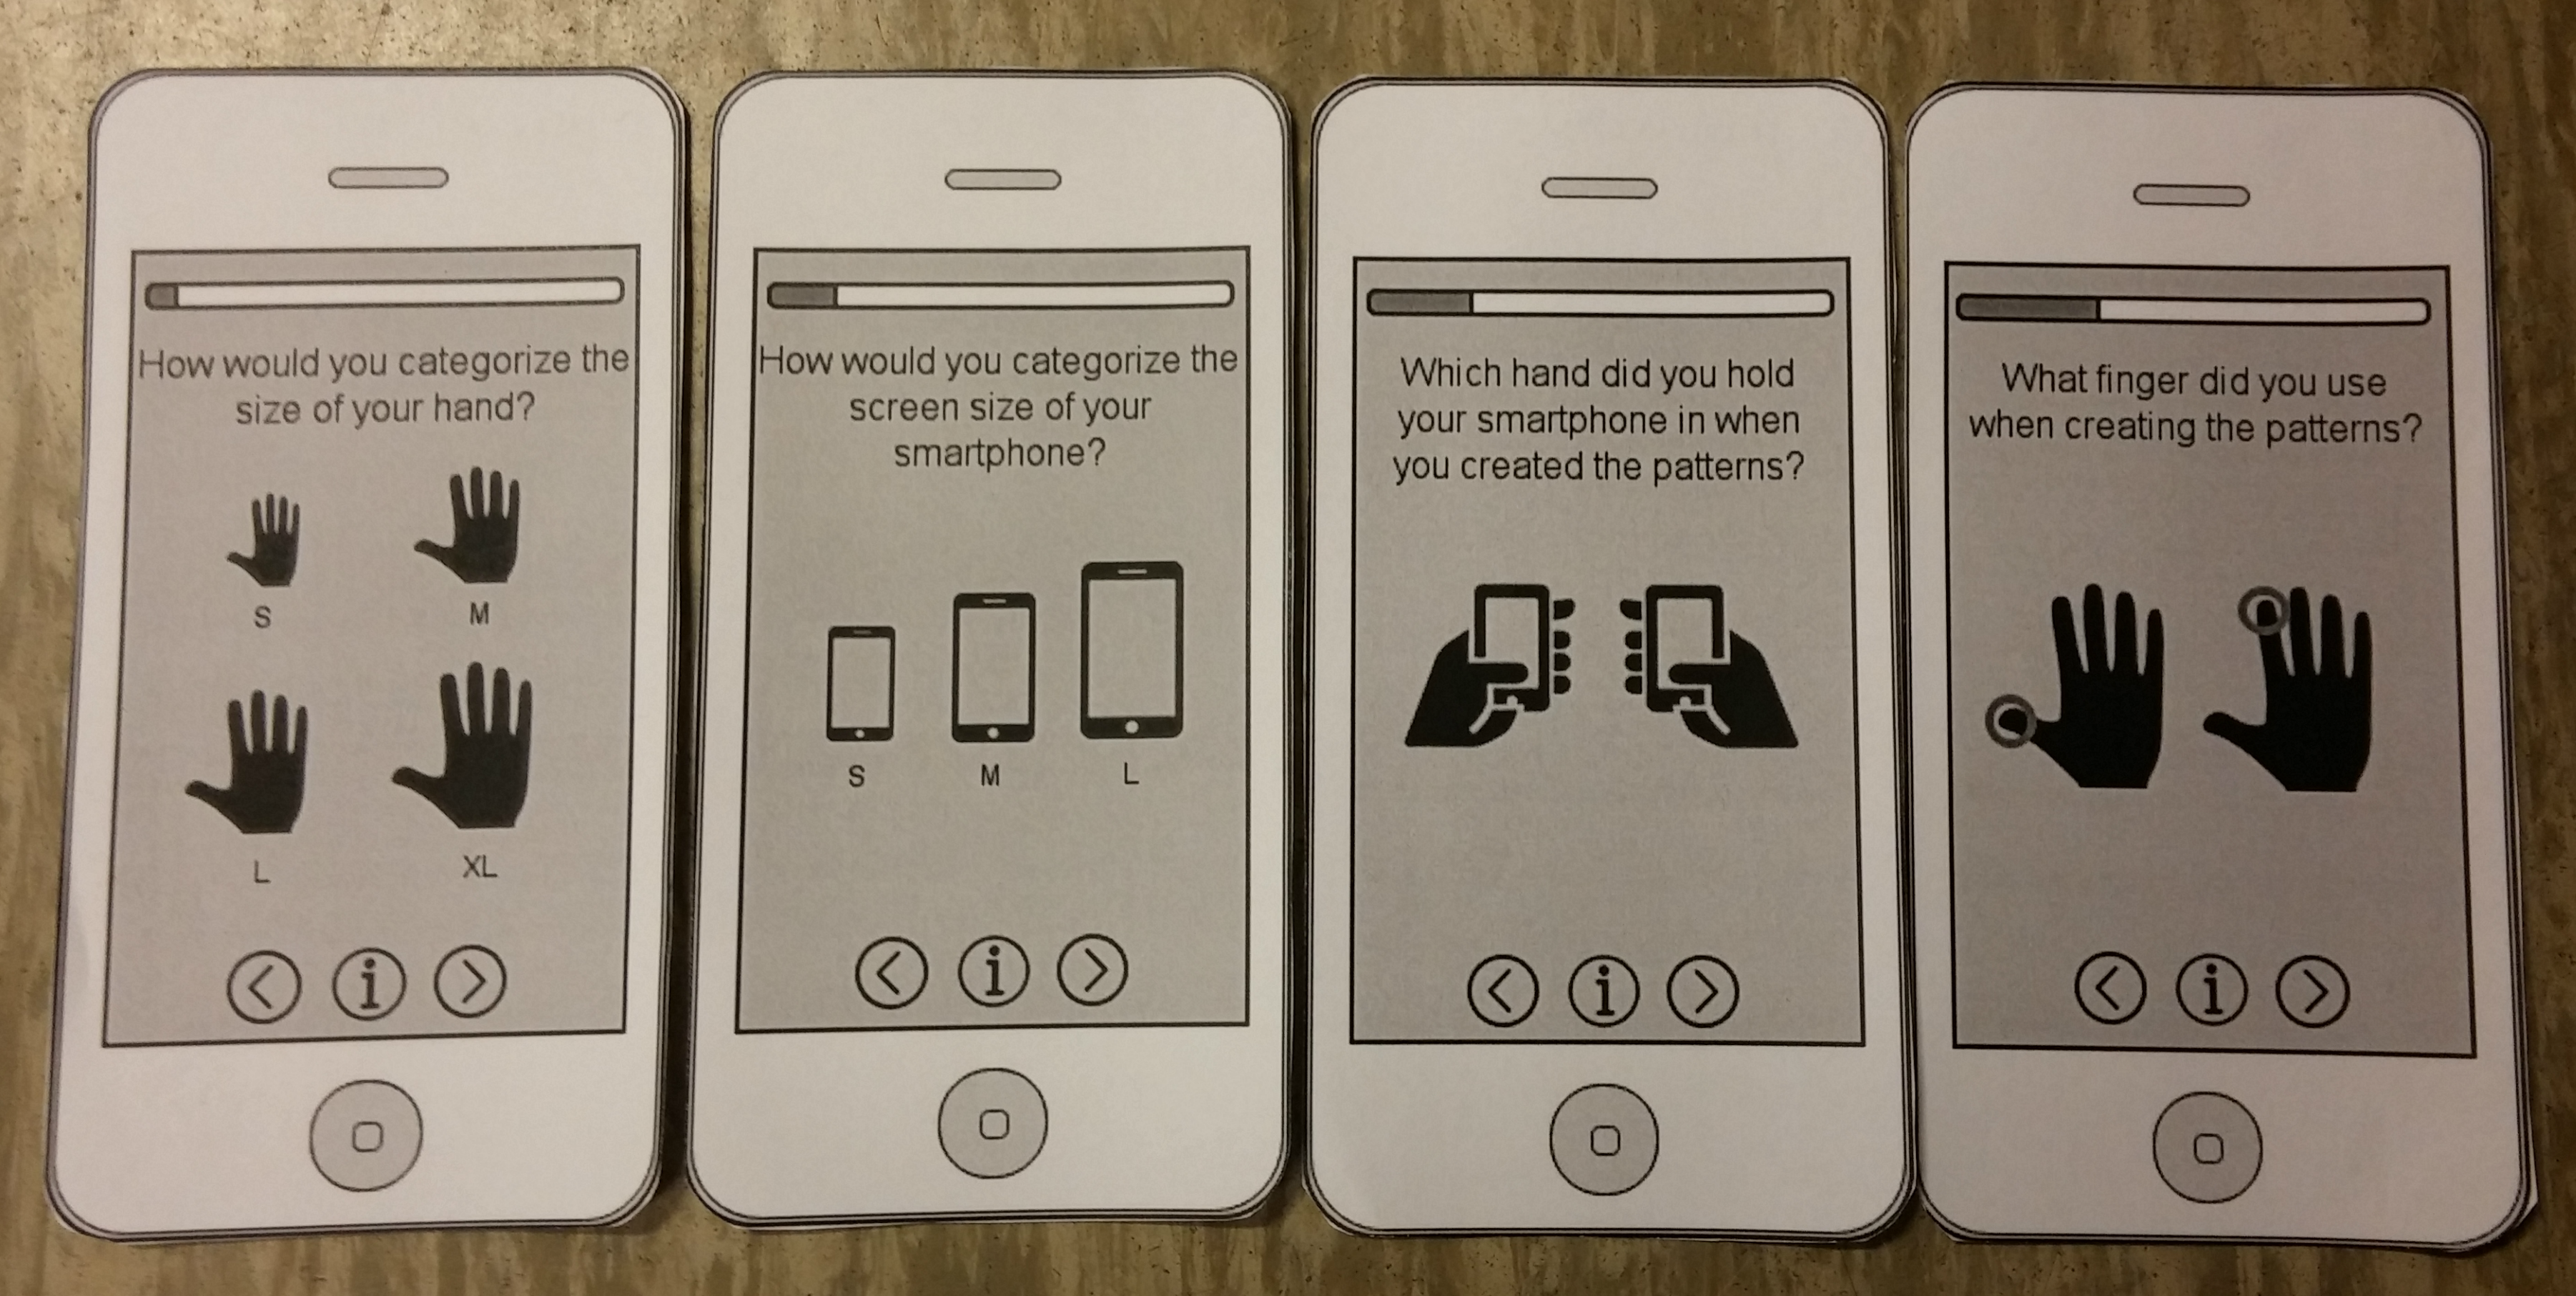
\includegraphics[width=\textwidth]{pics/test1.png}
      \caption{Usability test 1}
      \label{fig:test1}
    \end{figure}

  In the second test, it only tested the effectiveness (measured in number of errors) by only looking at the icons. When showing the icons to the participant, the actual question was covered. The students that participated in the test was supposed to guess what was asked for and select their answer by only looking at the icons. When conducting this test, the goal was to be able to see if the icons was understandable. When sending out the questionnaire, it is important that respondent that are not fluent in English are able to answer the questions without be able to understand all the English words. It is also useful for respondents to be able to use the text and the icons together in order to understand the questions. Figure~\ref{fig:test2} is showing an image from test 2, where the question is covered. 

    \begin{figure}[H]
      \centering
      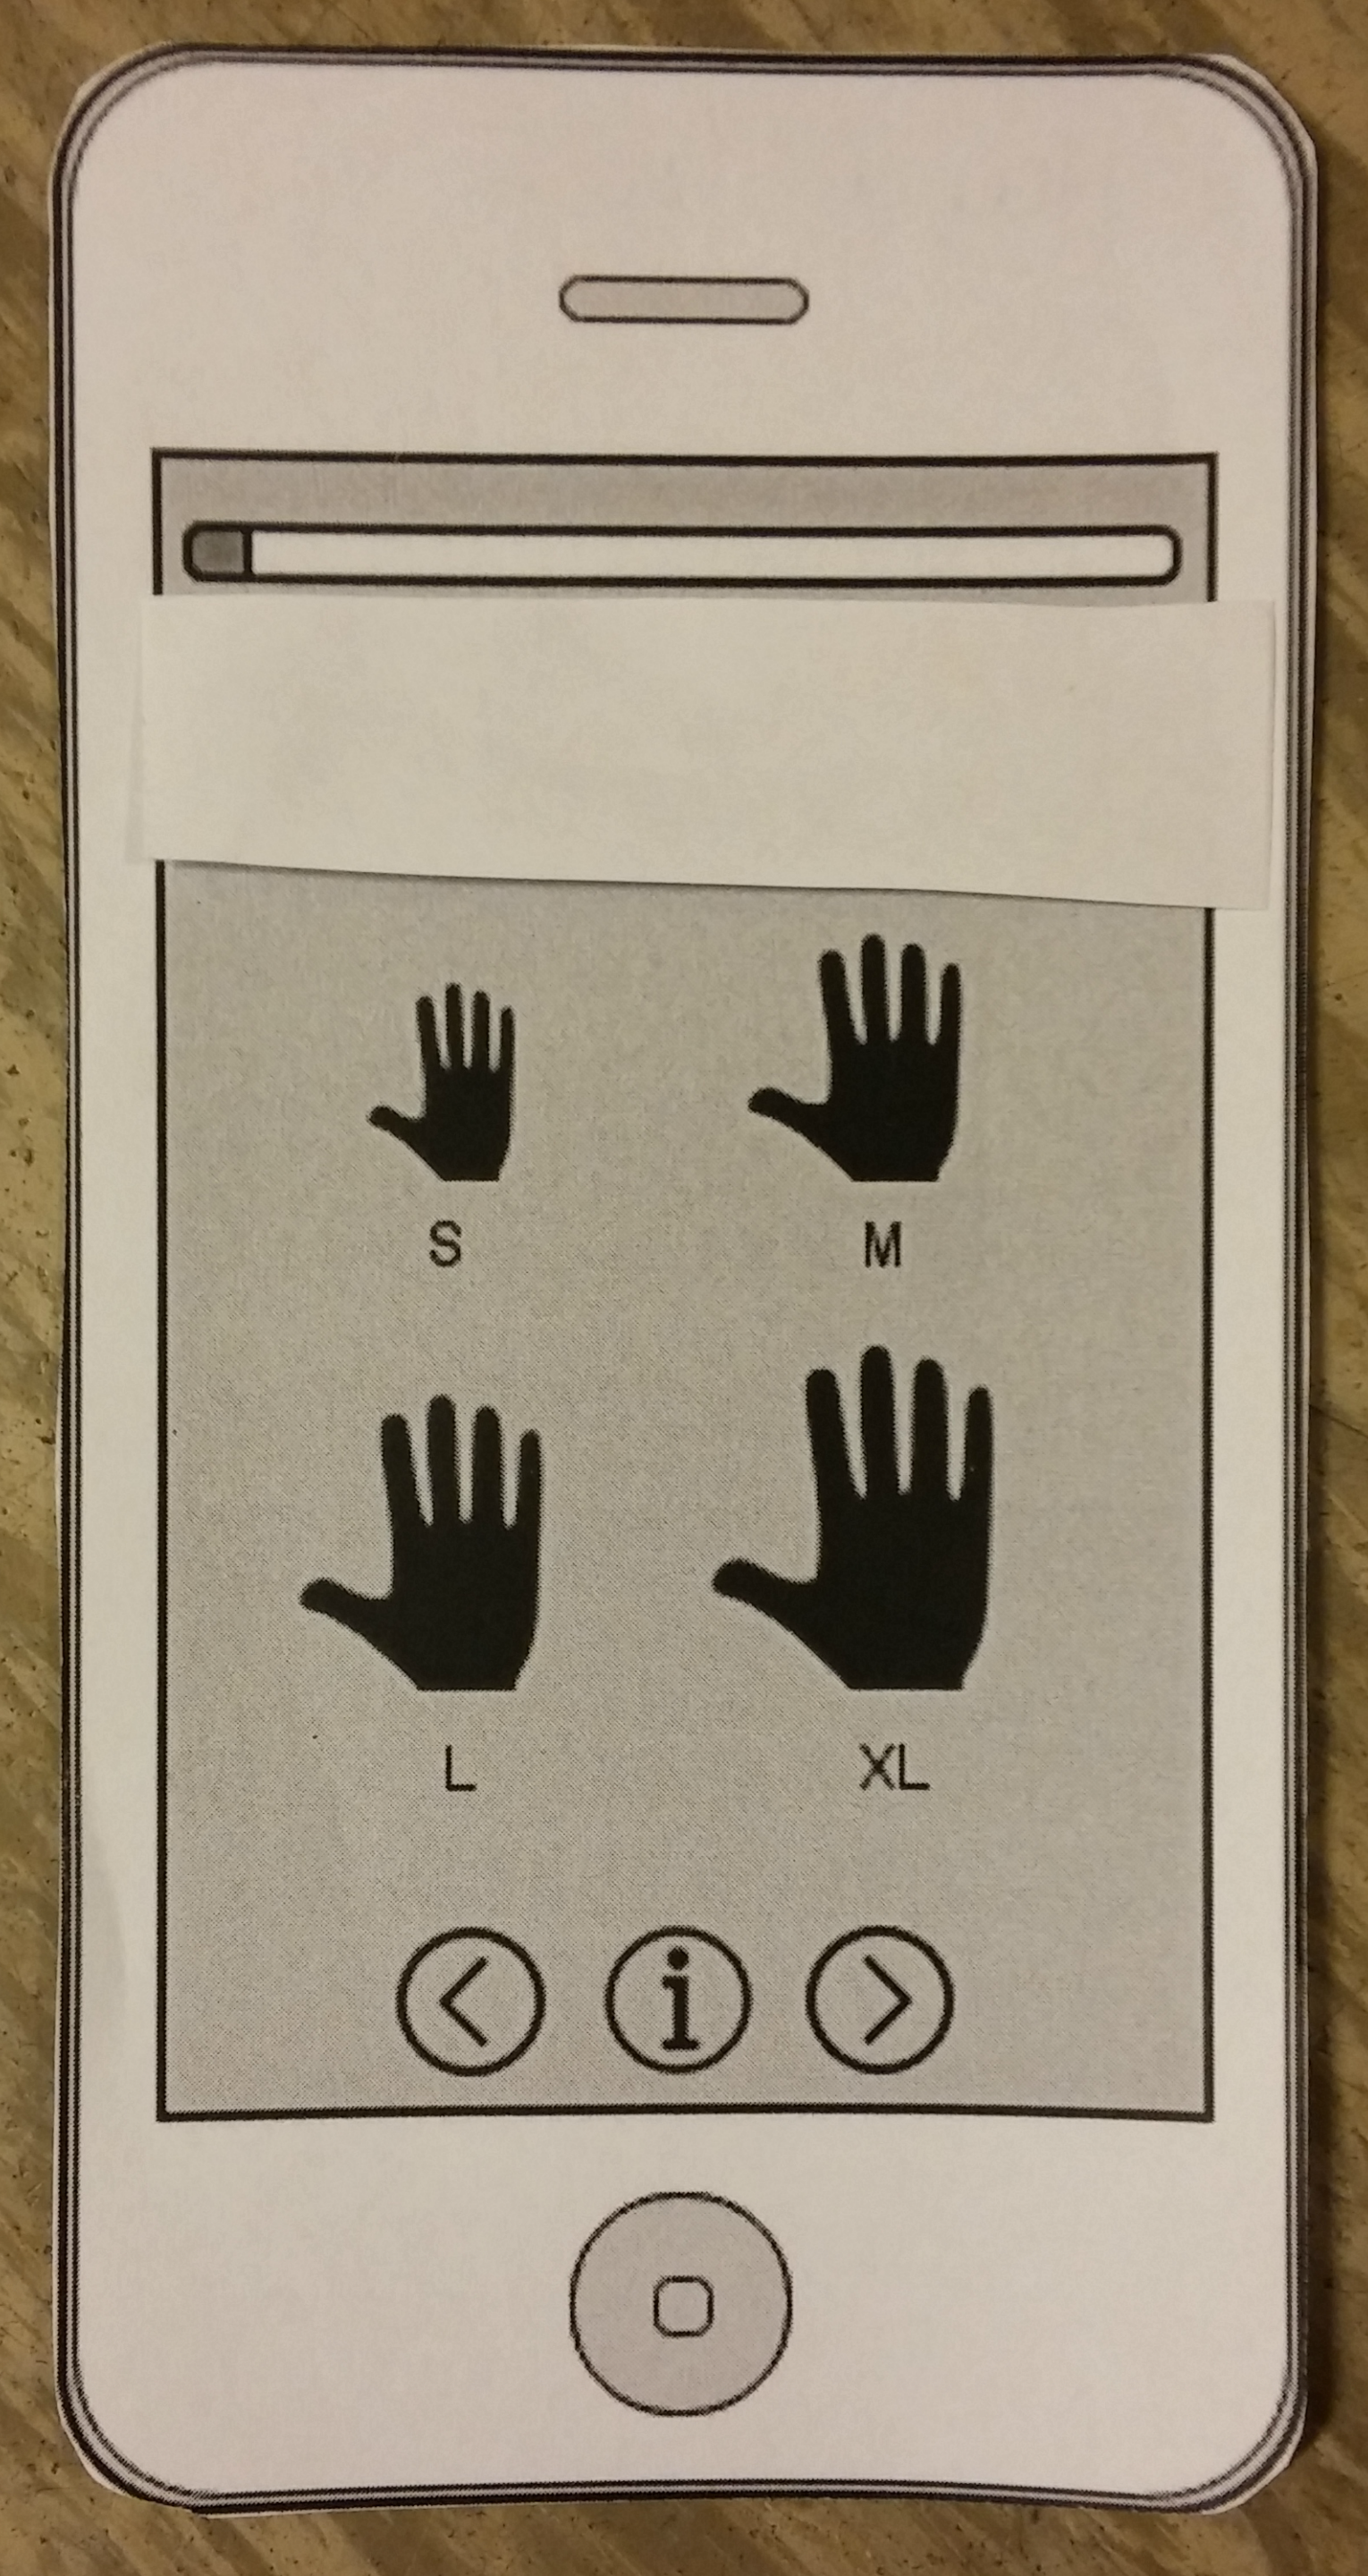
\includegraphics[scale=0.2]{pics/test2.png}
      \caption{Usability test 2}
      \label{fig:test2}
    \end{figure}

  \subsubsection*{Results}

  For testing the prototype, I contacted five girls and five boys (age from 20-24) from the university, resulting in 5 participants in each test. This is a small number of participants and does only represent a small part of the population. The primary goal was to get some feedback on the wireframes from Section~\ref{fig:wireframes}. The participants were explained that the test did not test their knowledge, rather the systems and its design. If they ever felt uncomfortable, they were also told that they could quit the test whenever they wanted. The feedback from the participants will be included in the next version of the prototype. The new prototype will be tested and implemented next semester.

  In test 1, all the wireframes were used and was demonstrated in the same order as Figure~\ref{fig:wireframes}. Before they started on the questionnaire, they were given information about the research, their right to stay anonymous, and the purpose of the research. The participants began when they pressed ``Start'' as illustrated in Figure~\ref{fig:wireframe1}. During the test, the participants commented on some part of the test.

  {\bf Comment on Figure~\ref{fig:wireframe20}}: {\it "I study, but I have not finished my studies. Should I press yes?"}. All of the respondents was unsure whether to select "yes" or "no" in order to answer the question about their experience with IT and security. All the participants were IT-students, and all was unsure if the word ``studied'' was fitting their situation since they still were students. Most of the students chose to select ``no'' as their answers, but I would probably categorize all of them in a group experienced with IT and/or security. This question should be rephrased in order to avoid respondents to get in the same position.

  {\bf Comment on Figure~\ref{fig:wireframe12}}: {\it "What do you mean by reading and writing orientation?"}. One of the students were unsure what the question asked. The student guessed that the question posed for the direction that he used to write, but he got unsure when he read the ``top-to-bottom'' alternative because he could not relate to the alternative. He then clicked on the information button, and I explained what the different reading orientation was.

  {\bf Comment on the progress bar}: The progress bar in the prototype is very simple, and do not indicate how many questions that is left. Only one participant commented on this. He would like to see exactly how many questions that was answered and how many questions that is left. He suggested that he it could be used dots that are often used together with swipe navigation. He also added that this probably would be hard to implement because of the number of questions. An alternative suggestion was to remove the information icon next to the question and replace it with the number of questions answers (for example 2/12, two out of twelve questions answered).

  {\bf Comment about the pattern creation}: {\it "I would like to create a pattern for the smartphone first because I wanted to use the pattern from my own smartphone because that is something I am familiar with"}.

  After the participants completed the question, I asked a set questions:

  {\bf Question 1 - Navigation}: All the participants were asked how they felt about the flow and navigation in the system. The reason this question is asked is because the prototype has two arrows that are indicating how to get to the next question. On mobile devices, it is desirable to have the least possible amount of clicks in order to use less time. Pressing the same button to go to the next question can for some users be annoying. The arrows are added to the prototype because it is hard to simulate automatic animation or swipe navigation on paper. The participants got a chance to express how they would like the navigation to be, and how they would expect it to work. All the respondents would like the questions to navigate automatically when they selected their answers. Some of the participants commented that they wanted the icons to change color, and then see an animation of the automatic animation. Some of the participants that wanted the automatic navigation added the comment that they wanted to be able to go back if they chose the wrong answer. So if the automatic navigation was added, then there was a need to be able to go back, so they did not lose control. Two of the respondents wanted the questionnaire to support swipe navigation because they expect that this is how website navigation works.

  {\bf Question 2 - Trustworthiness}: All the respondents were asked if they felt confident when they answered the questionnaire. Asking people to give away patterns might result in loosing some respondents because they do not feel confident. It is, therefore, important to provide enough information about the research and how the data is going to be used. The trustworthiness is important to obtain from the respondents already in the introduction. 

  In test 2, the respondents were challenged with the wireframes that contained icons. They guessed what was asked for and then selected they answer with an explanation of why they did so. All the five respondents (three girls and two boys) managed to interpret the icons and guess most of the questions. There was one participant that guessed that the wireframe in Figure~\ref{fig:wireframe16} was asking if they used the Android scheme. It is quite close, but not the exact question. I do not see this as a problem because all the respondents from test 1 manage to interpret the question correctly. One drawback with this test is that the icons are quite simple, and some of them might not be good enough for the actual implementation. 

  The results from both tests is providing important information that will be used to make suggestions for redesign. The Suggested improvements is further described as suggestions in the chapter for further work. 
